% 三角函数(高中)
% keys 高中|三角函数
% license Usr
% type Tutor
\pentry{弧度制与任意角\nref{nod_HsAngl},几何与解析几何初步\nref{nod_HsGeBa},函数\nref{nod_functi},函数的性质\nref{nod_HsFunC},导数\nref{nod_HsDerv}}{nod_1829}
\begin{issues}
\issueDraft
\end{issues}

在初中阶段,三角函数通常是在\aref{直角三角形的背景下}{eq_HsGeBa_1}引入的。在学习时,相信读者尚未学习“函数”这一概念,自然仅仅将其作为名称接受,并未意识到它与数学上的函数有何关联。而现在,在了解了函数表示的是输入与输出之间的确定关系的基础上,回顾初中的学习内容,可以发现:无论直角三角形的边长如何变化,只要其中一个锐角固定,三边之间的任意两者的比例始终不变。这一现象正是函数关系的体现——每个角都对应着唯一的比例,这也解释了三角函数名称的由来。

三角函数是一个历史悠久的数学主题,它的独特性在于,它不仅直接关联于几何图形,同时也符合函数的数学定义。这种双重属性使其从一开始就展现出复杂性。然而,复杂性往往伴随着强大的应用能力——事实上,几乎所有的周期函数都可以用三角函数表示。这一特性催生了一门重要的数学分支——\textbf{傅里叶分析(Fourier analysis)},它构成了现代电子信息技术、信号处理等领域的基础,建立了时间与频率之间的数学联系。

随着角度的推广,三角函数的定义不再局限于直角三角形,而是扩展到任意角,并引入弧度制,使角度能够以实数的形式表示,从而与当前学习的实数函数体系结合,使角度成为三角函数的自变量。尽管在几何问题中仍然使用角度作为标记,但在涉及函数视角的导数等运算时,通常采用弧度制。例如,在弧度制下,$\sin x$ 在 $x=0$ 处的导数为 $1$,这一性质在微积分中具有重要意义,使得数学运算更加简洁自然。

\subsection{任意角下的三角函数}
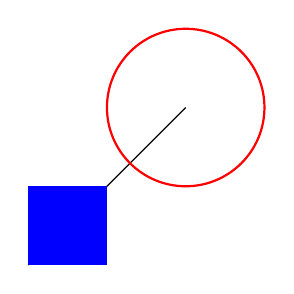
\begin{tikzpicture}
    \draw (0,0) -- (2,2);  % 画一条直线
    \draw[red, thick] (2,2) circle (1cm); % 画一个红色的粗圆
    \fill[blue] (0,0) rectangle (1,1);  % 画一个填充蓝色的矩形
\end{tikzpicture}
我们取单位圆上一点 $P(u,v)$,令 $OP$ 与 $x$ 轴夹角为 $\alpha$,则 
\begin{equation}
\begin{aligned}
\cos\alpha &= u,\\
\sin\alpha &= v,\\
\tan\alpha &= \frac{v}{u}~.
\end{aligned}
\end{equation}
\begin{figure}[ht]
\centering
\includegraphics[width=10cm]{./figures/82d1d7f3babb1847.png}
\caption{如图所示} \label{fig_HsTrFu_3}
\end{figure}
易得,正弦函数和余弦函数的\textbf{定义域为全体实数},正切函数的定义域为 $\begin{Bmatrix}\alpha|\alpha \neq \frac{\pi}{2}+k\pi,k\in Z\end{Bmatrix}~.$

\subsection{三角函数的性质}

\subsubsection{周期性}
正弦函数、余弦函数、正切函数的都是周期函数,根据定义易得,正弦函数和余弦函数,周期为 $2k\pi(k\in Z,k\neq0)$,正切函数的周期为 $k\pi(k\in Z,k\neq0)$.
\subsubsection{导数}

\subsection{图像}

\begin{figure}[ht]
\centering
\includegraphics[width=14.25cm]{./figures/bb986656153a547d.png}
\caption{正弦函数} \label{fig_HsTrFu_1}
\end{figure}
\begin{figure}[ht]
\centering
\includegraphics[width=14.25cm]{./figures/d0ae1e0d9c167f1e.png}
\caption{余弦函数} \label{fig_HsTrFu_2}
\end{figure}
可以看出正弦函数和余弦函数是定义域为 $R$ 值域为 $[-1,1]$ 最小正周期 $T = 2\pi$ 的周期函数。

\subsection{*同角三角函数的基本关系}
三角函数除以上介绍的三种,还有三种:
\begin{enumerate}
\item 正割函数 \textbf{\textsl{sec α}} 
\begin{equation}
\sec \alpha = \frac{r}{u}~.
\end{equation}
(这里的 “r” 指上文OP的距离)
\item 余割函数 \textbf{\textsl{csc α}} 
\begin{equation}
\csc \alpha = \frac{r}{v}~.
\end{equation}
\item 余切函数 \textbf{\textsl{cot α}} 
\begin{equation}
\cot \alpha = \frac{u}{v}~.
\end{equation}
\end{enumerate}
了解三种函数后,同角三角函数的基本关系符合以下图示:
\begin{figure}[ht]
\centering
\includegraphics[width=12cm]{./figures/6390d1e662067a9b.png}
\caption{同角三角函数的基本关系} \label{fig_HsTrFu_4}
\end{figure}
\begin{itemize}
\item 三角函数倒数关系:
\begin{equation}
\tan \alpha  \cot \alpha = 1~,
\end{equation}
\begin{equation}
\sin \alpha  \csc \alpha = 1~,
\end{equation}
\begin{equation}
\sec \alpha  \cos \alpha = 1~.
\end{equation}
可以发现这个关系是六边形的对角线。
\item 三角函数商数关系:
\begin{equation}
\tan \alpha = \frac{\sin \alpha}{\cos \alpha}~,
\end{equation}
\begin{equation}
\cot \alpha = \frac{\cos \alpha}{\sin \alpha}~.
\end{equation}
剩下的不做列举
可以发现这个关系是:顶点函数值等于相邻两顶点乘积
\item 三角函数平方关系:
\begin{equation}
\sin ^{2} \alpha + \cos ^{2}\alpha =1~,
\end{equation}
\begin{equation}
\tan  ^{2} \alpha + 1 =\sec ^{2}\alpha~,
\end{equation}
\begin{equation}
1 + \cot ^{2}\alpha =\csc ^{2}\alpha~.
\end{equation}
可以发现这个关系按照图示颜色三角形进行。
\end{itemize}
